% Diese Zeile bitte -nicht- aendern.
\documentclass[course=erap]{aspdoc}

%%%%%%%%%%%%%%%%%%%%%%%%%%%%%%%%%
%% TODO: Ersetzen Sie in den folgenden Zeilen die entsprechenden -Texte-
%% mit den richtigen Werten.
\newcommand{\theGroup}{151} % Beispiel: 42
\newcommand{\theNumber}{A324} % Beispiel: A123
\usepackage{graphicx}
\graphicspath{ {./images/} }
\author{Aaron Schulze \and Kerem Colak \and Ignat Kharlamov}
\date{Wintersemester 2022/23} % Beispiel: Wintersemester 2019/20
%%%%%%%%%%%%%%%%%%%%%%%%%%%%%%%%%

% Diese Zeile bitte -nicht- aendern.
\title{Gruppe \theGroup{} -- Abgabe zu Aufgabe \theNumber}

\begin{document}
\maketitle

\section{Einleitung}

Das Berechnen von Primzahlen ist ein wichtiges Teilgebiet der Zahlentheorie und damit auch der Informatik, dessen Untersuchung schon vor dem 3. Jahrhundert v. Chr. angefangen wurde. 
Eine Primzahl ist gemäß Definition eine ganze Zahl größer als 1, die außer 1 und sich selbst keine weiteren positiven Teiler hat. \cite{Weitz2018} 
Der Begriff stammt aus dem lateinischem ''numerus primus'', was mit ''die erste Zahl'' übersetzt werden kann. \cite{zenoDictionary} 
Mit ''primus'' bezieht man sich insbesondere auf ''den Anfang, das Erste (der Dinge)'', also eine Anfangszahl, die nicht aus anderen natürlichen Zahlen zusammengesetzt ist, 
die jedoch durch Multiplikation mit anderen Faktoren unendlich viele weitere natürliche Zahlen erzeugen kann.
\\Diese ist nur eine der vielen Eigenschaften von Primzahlen, die sich in der Informatik als sehr nützlich erweisen. Insbesondere werden in der Kryptographie häufig Primzahlgeneratoren verwendet, 
um auf effiziente Weise geheime Schlüssel zu generieren, die allerdings auf keine effiziente Art wiederhergestellt werden können. 
Das RSA-Verschlüsselungsverfahren, was heute als Standard für die Verschlüsselung geheimer Nachrichten verwendet wird, ist ein Beispiel davon. 
Bei diesem Verfahren wird der Schlüssel durch die Multiplikation zweier (großer) Primzahlen ausgerechnet. Die Stärke dieses Verfahrens basiert sich auf die Tatsache, 
dass die Primfaktorzerlegung einer Zahl (in diesem Fall der geheime Schlüssel) mit den heutigen bekannten Methoden nicht praktisch durchführbar ist.\\Es gibt noch zahlreiche Beispiele für praktische Anwendungen von Primzahlen: andere Kryptografische Verfahren, Fehlerkorrekturverfahren, Zufallszahlengeneratoren und weitere.
Dies soll die Bedeutung der Primzahlen verdeutlichen. Bereits in der Vergangenheit wurden zur Generierung von Primzahlen Algorithmen entwickelt 
und mathematische Sätze formuliert, die auch heute relevant sind.
Die Schwierigkeit, die sich beim Berechnen von Primzahlen ergibt, zusammen mit ihren starken Eigenschaften, ist gleichzeitig der Grund, weshalb diese auch in zahlreiche Gebiete 
der Informatik eingesetzt werden. Unser Projekt beschäftigt sich mit dem Teil über die Primzahlberechnung; insbesondere sollten unterschiedliche Algorithmen umgesetzt werden, die in der Lage sind, die ersten \textit{n} Primzahlen zu berechnen und in einem Array zu speichern.
Diese Ausarbeitung wird sich im Weiteren mit verschiedene Ansätze für die Generierung von Primzahlen beschäftigen. 
\section{Lösungsansatz}
\subsection{Die Methode der Probedivision}
Für die Berechnung der ersten \textit{n} Primzahlen kann man sich erstmal einen naiven\\ Algorithmus ausdenken, der auf den ersten Blick intuitiv sein mag.
\\Gemäß dem Fundamentalsatz der Arithmetik lässt sich jede natürliche Zahl \textit{n} > 1 als Produkt endlich vieler Primzahlen darstellen \cite{TheoremDavidBurton2011}. 
Wenn man also überprüfen möchte, ob die \textit{k}-te Zahl prim ist, für $k \in \{2,...,n\}$, dann ist es hinreichend zu prüfen, ob sich diese Zahl als Produkt irgendwelcher kleineren Faktoren schreiben lässt. Man überprüft also durch die Modulo-Division, ob \textit{k} irgendeinen Teiler hat, der nicht 1 oder die Zahl selbst ist. Falls dies der Fall ist, dann ist die Zahl zusammengesetzt und damit keine Primzahl. Diese Überprüfung durch Modulo-Division muss für jede Zahl zwischen 2 und \textit{n} geschehen.
\\Dieser erster Ansatz, der auch als Methode der Probedivision bekannt ist, sollte allerdings nur als Intuition für die Berechnung von Primzahlen dienen. 
Es müssen nämlich (\textit{n}-1) Primzahltests ausgeführt werden, und für den \textit{k}-ten Primzahltest müssen alle Faktoren bis \textit{k} bzw. potenziell bis \textit{n} 
auf Restdivision überprüft werden.\\Eine konkrete Implementierung kann beispielsweise zwei verschachtelte Schleifen enthalten: eine die über alle Primzahlkandidaten von 2 bis  \textit{n} iteriert 
und eine innere Schleife, die für alle kleinere Faktoren eine Probedivision ausführt. Dies führt zu einer Laufzeit des Algorithmus von
$\mathcal{O}(n^2)$. Diese einfache Methode kann allerdings noch weiter optimiert werden.
Beim \textit{k}-ten Primzahltest, für $k \in \{2,...,n\}$, ist es hinreichend nur die bisher gefundenen Primfaktoren zu betrachten, anstatt aller natürlicher Zahlen zwischen 2 und \textit{k}. Damit kann man die Tatsache ausnutzen, dass man alle vorherigen Primzahlen bis \textit{k} schon ausgerechnet hat, 
da alle andere mögliche Faktoren wiederrum in Primzahlen zerlegbar sein würden. Außerdem kann man sogar nur die Primfaktoren kleiner als $\sqrt{k}$
betrachten: ist nämlich ein Faktor von \textit{k} größer als $\sqrt{k}$, dann muss ein anderer Faktor kleiner als $\sqrt{k}$ sein, da sich am sonsten ein Widerspruch ergeben würde \cite{DavidBurton2011}. Durch diese Beobachtung wird die Kardinalität der Menge von Faktoren, die einen Primzahlkandidat zusammensetzen könnten, deutlich reduziert. Außerdem ist jede gerade Zahl bis auf die 2 eine zusammengesetzte Zahl, da sich jede gerade Zahl durch 2 teilen lässt. Das impliziert, dass keine gerade Zahl größer als 2 ein Kandidat für eine mögliche Primzahl sein kann. 
Also kann auch die Menge der Primzahlkandidaten halbiert werden.\\Ein kleines Beispiel um das ganze zu verdeutlichen: sei \textit{k} = 121, der Primzahlkandidat, mit $\sqrt{k} \approx 11$. Es wird nun überprüft, ob \textit{k} durch irgendeinen Primfaktor zwischen 2 und 11 teilbar ist. Durch die iterative Ausführung der Modulo-operation auf jeden Primfaktor stellt man fest, dass 121 durch die 11 teilbar ist, also ist 121 keine Primzahl. 
Trotz Optimierungen ist diese Methode für große Werte von \textit{n} nicht Praktikabel. 
Die innere Schleife tut die Laufzeit sehr stark beeinflussen, so dass schon bei $n>10^6$ die Laufzeit mehrere Minuten beträgt. 
Wir möchten allerdings in unserer Lösung auch größere Werte für \textit{n} annehmen können.
\subsection{Das Sieb des Eratosthenes}
Die Idee, die Anzahl der Elemente der zwei Mengen zu reduzieren, wird auch von einer der ältesten und einer der relevantesten Methoden 
verwendet. Diese Methode ist als das Sieb des Eratosthenes bekannt, nach dem griechischen Wissenschaftler Eratosthenes von Kyrene (276 – 194 v.Chr.). 
Die Methode selbst war schon lange vor Eratosthenes bekannt, allerdings war Eratosthenes der erste, der das Verfahren als ''Sieb'' bezeichnet hat. 
Wie der Name vermuten lässt, werden mit diesem Verfahren alle Primzahlkandidaten tatsächlich gesiebt, so dass am Schluss nur Primzahlen übrigbleiben, 
was sich genau für unser Problem für das Ermitteln von Primzahlen eignet.\\Das originale Verfahren des Siebs ermöglicht es, alle Primzahlen in einem Zahlenbereich von 2 bis \textit{n} zu finden. Im ersten Schritt werden alle natürlichen Zahlen zwischen 2 und \textit{n} aufgelistet oder in einer Tabelle dargestellt 
und zunächst als Primzahlen markiert. Am Anfang sind also alle Zahlen potenzielle Primzahlen. 
Der Algorithmus fängt bei der ersten Zahl an, d.h. die 2, die als Primzahl markiert ist. 
Jetzt werden sukzessive alle Vielfachen der 2 aus der Menge der markierten Primzahlen rausgestrichen, bis \textit{n} erreicht wird. 
Alle Vielfachen der 2 sind nämlich zusammengesetzte Zahlen und daher keine potenzielle Primzahlen. Dann wird die nächste Zahl genommen, 
die noch nicht gestrichen wurde: das ist die 3, welche auch unsere nächste gesuchte Primzahl ist. 
Es werden erneut alle Vielfachen der 3 gestrichen, bis \textit{n} erreicht wird. 
Damit sind alle Vielfachen der 2 und der 3 aus der Menge der Kandidatenzahlen gesiebt wurden, und werden im Weiteren nicht mehr betrachtet. Die 4 wird übersprungen, da sie als Vielfaches der 2 schon gestrichen wurde, und es werden alle Vielfachen der 5 gesiebt.  
Wenn man dieses Verfahren für alle Zahlen, die noch nicht gestrichen wurden, solange wiederholt bis \textit{n} erreicht wurde,
dann bleiben am Ende in der Liste oder in der Tabelle nur die Primzahlen zwischen 2 und \textit{n} übrig. Ein kleines Beispiel für die ersten zwei Iterationen: 
\begin{center} [2, 3, 4, 5, 6, 7, 8, 9, 10, 11, 12, 13, 14, 15, ..., 100] -  Anganfsbelegung \end{center}
\begin{center} [2, 3, {\color{red}4}, 5,  {\color{red}6}, 7, {\color{red}8}, 9,  {\color{red}10}, 11, {\color{red}12}, 13, {\color{red}14}, 15, ..., {\color{red}100}] - Vielfache der 2 \end{center}
\begin{center} [2, 3, {\color{red}4}, 5,  {\color{red}6}, 7, {\color{red}8}, {\color{red}9},  {\color{red}10}, 11, {\color{red}12}, 13, {\color{red}14}, {\color{red}15}, ..., {\color{red}100}] -  Vielfache der 3\end{center}
Das Sieb des Eratosthenes findet alle Primzahlen innerhalb eines bestimmten Bereiches. 
Beispielsweise gibt es zwischen 2 und 100 genau 25 Primzahlen, die im Sieb übrigbleiben. 
Bei unserem Problem geht es allerdings darum, die ersten \textit{n} Primzahlen zu generieren bzw. diese zu finden. 
Daher ist es nötig, den Suchbereich  über dem das Sieb ausgeführt wird sinnvoll zu begrenzen.\\
Dafür gibt es eine Formel, die eine Abschätzung für den Zahlenbereich liefert, in dem sich die ersten \textit{n} Primzahlen befinden, die folgendermaßen aussieht:$$p_n<n(\log n + \log\log n), n \geq 6$$ \begin{flushright} \cite{Axler} \end{flushright}
Dabei ist mit $p_n$ die \textit{n}-te Primzahl gemeint. Mit dieser Abschätzung haben wir eine obere Schranke für die \textit{n}-te Primzahl, 
so dass durch die Anpassung des Siebsbereiches nach Anwendung des Siebs die ersten \textit{n} Primzahlen gefunden werden.\\ Das Sieb hat trotz verbesserte Laufzeit noch einen großen Nachteil, 
nämlich der Speicherbedarf, der $\mathcal{O}(n)$ beträgt. 
Bei einer konkreten Implementierung kann man beispielsweise die Markierung der Primzahlkandidaten durch ein bool Array verwalten, 
so dass für jeden Primkandidat gespeichert werden kann, ob es sich um eine Primzahl oder um ein Vielfaches einer Primzahl handelt. 
Zu Beginn des Algorithmus sind alle Zahlen gleich markiert; die Markierung wird während der Ausführung entsprechend aktualisiert. 
Dazu muss ein array mit Speicherplatz für \textit{n} bool Werte reserviert werden; allerdings 
hat ein bool im Speicher gemäß C-Standard eine Größe von 1 Byte. 
Für große Werte von \textit{n} ist das problematisch, da ein sehr großer Speicherbereich durch ein Aufruf von \textit{malloc()} nicht mehr reserviert werden kann. Eine Möglichkeit, was dieses Problem lösen könnte, ist die Verwendung von einem Array was für die Verwaltung der Markierung nur bits speichert, beispielsweise eine 1 für eine Primzahl und eine 0 sonst. Selbst durch die Anwendung der mathematischen Optimierungen die im Abschnitt [2.1] erwähnt wurden, stellt der linearer Speicherbedarf ein Problem dar; es muss immer genügend freier Speicher vorliegen, damit der Algorithmus überhaupt ausgeführt werden kann. 
\subsection{Die Wormell'sche Formel}
Ein weiterer Ansatz, um die ersten \textit{n} Primzahlen zu berechnen, ist die Wormell’sche Formel, die uns in der Aufgabenstellung gegeben wurde und die folgendermaßen aussieht: $$
p_{n} = \frac{3}{2} + 2^{n - 1} - \frac{1}{2} \sum_{m=2}^{2^n} (-1)^{2^{\prod_{r=1}^{n} \left(1-r + \frac{m-1}{2} + \frac{1}{2} \sum_{x=2}^{m} (-1)^{2^{\prod_{a=2}^{x} \prod_{b=2}^{x} (x-ab)^2}}\right)^2}}
$$
Diese Formel ermöglicht es für eine Eingabe \textit{n} die \textit{n}-te Primzahl zu berechnen. Wenn man jetzt prüfen möchte, ob eine gegebene Zahl \textit{k} prim ist, dann könnte man sich durch diese Formel eine Folge der ersten Primzahlen generieren, die von 2 bis $\sqrt{k}$ gehen, um alle Primfaktoren zu kriegen die \textit{k} zusammensetzen könnten. Danach müsste man erneut \textit{k} mit den gefundenen Primfaktoren auf Restdivision prüfen. Allerdings ist es relativ offensichtlich, dass diese keine gute Lösung für die  Implementation eines Primzahltests ist: bei dieser Überprüfung, wird selbst nur die Generierung der Folge aufwendig sein, da für große Werte von \textit{n} ekzessive Schleifendurchläufe asugeführt werden müssen. Auch für die Berechnung der ersten \textit{n} Primzahlen lohnt es sich nicht diese Formel umzusetzen. Man kann zwar dank der Struktur der Formel ohne weitere Erkenntnisse über andere Primzahlen die \textit{n}-te Primzahl unmittelbar ausrechnen, so dass eine Folge von Primzahlen in linearer Weise konstruiert werden kann. Jedoch könnten bei einer naiver Implementierung welche die Formel eins zu eins übersetzt Performanzprobleme entstehen: \\ die äußerste Schleife läuft bis $2^n$, was schon bei sehr kleine Werte von \textit{n}
(\textit{n} < 100) zu einem Problem führt; außerdem gibt es mehrere verschachtelte innere Schleifen, die die Performanz stark beeinflussen. Aus diesen Gründen ist die Wormell'sche Formel für unsere Problemstellung nicht handhabbar. 
\subsection{SIMD Optimierungen}
Für die Anwendung von SIMD Instruktionen ist die Methode der Probedivision erstmal ungeeignet. 
Dieser Algorithmus basiert sich nämlich auf die Modulo Operation, für die es keine entsprechende SIMD Instruktion gibt.\\
Es wurde also versucht, SIMD Instruktionen auf das Sieb anzuwenden. Die erste Idee ist es, SIMD-Befehle für die Berechnung der Vielfachen einer gefundenen Primzahl zu verwenden, da das Sieb in diesem Abschnitt die meiste Rechenzeit verbringt. Wenn eine Primzahl durch das Sieb gefunden wird, dann werden die ersten 4 Vielfachen berechnet und in einem 256-bit AVX Vektor gespeichert. Sei als Beispiel die gefundene Primzahl \textit{p} = 7. Es müssen alle vielfachen größer als $7^2 = 49$ aus dem Sieb gestrichen werden, da alle Vielfachen kleiner als $\sqrt49$ schon gesiebt wurden. Der Vektor der Vielfachen ist wie folgt gefüllt: [7, 14, 21, 28]. Es können nur 4 Zahlen gespeichert werden, da jede Zahl 64 bit beträgt. Es wird dann ein ''Basisvektor'' gefüllt, mit dem Faktor ab dem die Vielfachen gestrichen werden sollen, d.h. [49, 49, 49, 49].\\Jetzt werden iterativ alle Vielfachen der 7 in 4er-Schritten ausgerechnet indem, die Basis und ein Offset addiert werden, so dass die Zahlen an den entsprechenden Indices aus dem Array für die Markierung gestrichen werden können. 
Der Offset ergibt sich aus einem Zähler der in 4er-Schritte inkrementiert wird: $offset = p \cdot counter$. 

\begin{center}
    [49, 49, 49, 49] + [7+0, 14+0, 21+0, 28+0]= [56, 63, 70, 77]
\end{center}
\begin{center}
[49, 49, 49, 49] + [7+28, 14+28, 21+28, 28+28] = [84, 91, 98, 105]
\end{center}
\begin{center}
[49, 49, 49, 49] + [7+56, 14+56, 21+56, 28+56] = [112, 119, 126, 133]
\end{center} Mit diesem Lösungsansatz werden werden zwar die Indices auf korrekter Weise ausgerechnet, allerdings hat sich kein Performanzgewinn ergeben; das originale Sieb ist sogar besser. Das liegt vermutlich an der erhöhter Anzahl an erforderlichen Speicherzugriffe um die Ergebniße der SIMD Addition zu lesen, und es werden viele Indices neu berechnet, obwohl diese von einer kleineren Primzahl schon gestrichen wurden (wie im obigen Beispiel für die Vielfachen der 2 zu sehen ist). Außerdem wird das Problem mit dem Speicherbedarf nicht gelöst\\
SIMD Instruktionen bieten auch die Möglichkeit an, auf Bit-Ebene zu arbeiten, so dass in der nächsten Implementierung versucht wurde die Markierung der Primzahlen in einem Array von Bits zu verwalten. Es werden also mehrere 128-Bit-Vektoren verwendet, wobei jedes Bit anzeigt, ob eine Zahl Prim ist oder nicht. Es wird im Nachinein angenommen, dass für unser \textit{n} erstmal ein einziger 128-Bit-Vektor ausreichend ist, um das Sieb ausführen zu können.  Dieser wird folgendermaßen initialisiert: \begin{center}[1,1,1,1,1,1, …,1] - Siebvektor\end{center}
Dabei steht eine 1 jeweils für eine potentielle Primzahl zwischen 2 und 130.
Dieser Vektor muss nach dem Verfahren des Siebs entsprechend aktualisiert werden, so dass nach Ausführung des Algorithmus jedes gesetzte Bit für eine Primzahl steht. Um die Bits aus den Vektoren zu entfernen, die ein Vielfaches einer Primzahl darstellen, wird ein 128-Bit-Offset erstellt, bei dem eine 1 an der Stelle der aktuellen Primzahl steht. Der Offset so wird initialisiert, dass bei die 2 die Bit-Markierung angefangen wird, d.h.,  \begin{center} [1,0,0,0,0,0,...,0]  - Offsetvektor, p=2 \end{center}
Um die Vielfachen zu streichen, wird der Offsetvetkor um k Stellen nach links verschoben, wobei k die von uns gefundene Primzahl ist, und es wird die logische Negation davon gebildet: 
\begin{center} [1,1,0,1,1,1,...,1]  - Offsetvektor \end{center} Danach wird eine AND-Operation mit dem Siebvektor ausgeführt und das Ergebnis im Siebvektor gespeichert, um das erste Vielfache zu streichen: \begin{center}[1,1,1,1,1,…,1] -  Siebvektor\end{center} \begin{center}[1,1,0,1,1,…,1] - Offsetvektor \end{center} \begin{center}[1,1,0,1,1,…,1] -  Ergebnis\end{center}
Die Operationen der Verschiebung um k Stellen, der Negierung und der Verundung mit dem Siebvektor, werden solange ausgeführt bis die letzte Zahl erreicht wurde, die gestrichen werden sollte. Wenn also alle Vielfachen der 2 gestrichen wurden, ist der Siebvektor wie folgendermaßen belegt: 
\begin{center}[1,1,{\color{red}0},1,{\color{red}0},1,{\color{red}0},1,…,{\color{red}0}] -  Siebvektor\end{center}
Der Offsetvektor wird nun auf seiner Initialbelegung zurückgesetzt: [1,0,0,0,0,0,...,0] - um eine Stelle verschoben: [0,1,0,0,0,0,...,0] - und mit den aktuellen Siebvektor verundet, so dass die 1 im Ergebnisvektor die aktuelle gefundene Primzahl darstellt, in diesem Fall die 3: [0,1,0,0,0,0,...,0]. Danach wird erneut der Offsetvektor um k = 3 Stellen nach links verschoben, und es werden iterativ die Vielfachen der 3 aus dem Siebvektor durch die AND-Operation gestrichen: \begin{center}[1,1,0,1,0,1,0,{\color{red}0},…,0] -  Siebvektor\end{center}
Letzendlich wird ein Array von \_\_m128i SIMD Vektoren verwendet, und der obige Prozess wird so lange wiederholt, bis alle Vektoren im Array durchgelaufen wurden sind. 
Dieser Ansatz löst das Problem des Speicherbedarfs der sich beim originalem Sieb ergibt, da nur n / (128+1) Vektoren gespeichert werden anstatt n 64-bit Zahlen. Dies ermöglicht es uns, noch höhere Werte für n annehmen zu können. Trotz Speicheroptimierung wird die Laufzeit nicht wesentlich schneller verglichen zur linearen Implementierung des Siebs, da die Generierung einer Maske für jeden einzelnen SIMD-Vektor erforderlich ist, was die Laufzeit immer noch stark beeinflusst. 
\section{Korrektheit}
In diesem Abschnitt möchten wir uns mit der Analyse der Korrektheit unserer Implementierung beschäftigen, 
da die Ergebnisse der Implementierung in konkrete Programmabläufe deterministisch und daher auf Korrektheit prüfbar sind. 
Die Implementierungsgenauigkeit wird hier nicht untersucht. 
Das Programm eignet sich nicht zum Vergleichen von Ergebnissen mit Abweichungen oder ähnliches.\\ 
Das Programm wurde um 19:00 Uhr am 02-01-2023 auf der Rechnerhalle in dem Ordner '/Implementierung' via SSH kompiliert und getestet. Es stehen außerdem folgende Implementierungsversionen zur Verfügung: V0 - das Sieb (Hauptimplementierung); V1 - Probedivision; V2 - Sieb mit SIMD und Bit-Vektoren; V3 - Sieb mit SIMD. Es wird erst das Rahmenprogramm getestet. Alle verfügbare Optionen werden von das Rahmenprogramm auf korrekterweise erkannt und bearbeitet. Wird das Programm beispielsweise mit ''./prim -n 100 -V0 -B5'' ausgeführt, dann werden die entsprechende Zahlenstrings
korrekt umgewandelt und die Variablen gesetzt. Um einige Randfälle zu testen, wird versucht ein String zu übergeben, welches keine vollständige Zahl beinhaltet: die Ausführung von './prim -n 123a' beendet mit einer Fehlermeldung über das falsche Format der Eingabe: ''Could not convert input string '123a' to integer.''
Die Verwendung von ungültige Optionen wie ''./prim -A'' beendet sich mit einer Fehlermeldung: ''The option char 'A' has a missing input parameter or is an invalid option.'' Es gibt noch zahlreiche Randfälle die beim Testen des Rahmenprogramms geprüft werden sollten, allerdings werden diese hier nicht betrachtet und es wird angenommen, dass das Rahmenprogramm korrekt ist. Es wird also die eigentliche Funktionalität des Programms untersucht. 
Unsere Funktion soll die ersten \textit{n} Primzahlen berechnen und diese in das Array 'prims[n]' reinschreiben. Zur Überprüfung der Korrektheit werden die Zahlen des Arrays mit offiziellen Primzahlen verglichen. Um die Ausgabe übersichtlich zu behalten, wählen wir erstmal einen kleinen Wert für \textit{n}; sei in diesem Beispiel \textit{n} = 20. Das Programm wird jetzt mit ''./prim -n 20 -P'' für die jeweiligen Versionen ausgeführt, wobei die Option 'P' die Inhalte des Arrays auf \textit{stdout} ausgibt. \\
Für jede der vier Auswählbaren Versionen ist die Ausgabe gleich, die folgendermaßen aussieht: \begin{center} [2, 3, 5, 7, 11, 13, 17, 19, 23, 29, 31, 37, 41, 43, 47, 53, 59, 61, 67, 71] \end{center}
Diese wird nun mit einer Liste von offiziellen Primzahlen verglichen, aus der wir die erste 20 wählen:
 \begin{center} [2, 3, 5, 7, 11, 13, 17, 19, 23, 29, 31, 37, 41, 43, 47, 53, 59, 61, 67, 71]\end{center} \begin{flushright}\cite[PrimesUtmEdu]{utmPrimes} \end{flushright}
 Offensichtlich sind die Werte übereinstimmend. Unter der Annahme, dass die Quelle der Werte vertraulich ist, sind also auch unsere Implementierungen in der Lage die ersten 20 Primzahlen korrekterweise zu berechnen. \\
 Für größere Werte von \textit{n} wird die Ausgabe des ganzen Arrays unübersichtlich, so dass die Möglichkeit besteht, dass man konkrete Werte die eigentlich falsch sind nicht mehr erkennt. Deshalb wird ab hier nur die \textit{n}-te Primzahl ausgegeben, die wiederrum mit einem offiziellen Wert verglichen wird. Bei unsere Verfahren ist die Berechnung der \textit{n}-ten Primzahl abhängig von der korrekter Berechnung aller Primzahlen bis (\textit{n}-1). Das impliziert, dass wenn die \textit{n}-te berechnete Primzahl korrekt ist, dann gilt dies auch für alle Primzahlen bis (\textit{n}-1); wäre dies nicht der Fall, dann wäre auch der Wert für die \textit{n}-te Primzahl falsch. Durch dieses Argument kann die Korrektheit aller Primzahlen bis zur \textit{n}-ten gewährleistet werden. Sei also zum Beispiel \textit{n} = 1'000'000. Es wird nochmal das Programm für alle Versionen von V0 bis V4 ausgeführt und die \textit{n}-te gespeicherte Primzahl ausgegeben. Das Ergebnis sieht für alle vier der Versionen folgendermaßen aus: \begin{center} prims\_array[n] = 15485863 \end{center}
 Dabei ist ein offizieller Wert der folgende: \begin{center} $p_n = 15485863$ \end{center}
 \begin{flushright}\cite[WolframAlpha]{wAlpha1} \end{flushright}
 Damit ist auch für dieser Wert von \textit{n} die Berechnung der Primzahlen korrekt. Für noch größere Werte terminiert die Methode der Probedivision nicht, und wird im Weiteren vernachlässigt. Allerdings möchten wir noch die andere Verfahren auf Korrektheit weiterprüfen. Sei also jetzt \textit{n} = 100'000'000, für V0, V2, V3. Es wird nochmal auf Korrektheit geprüft: \begin{center} prims\_array[n] = 2038074743 \end{center} Der offizielle Wert ist übereinstimmend mit das Ergebnis des Programms: \begin{center} $p_n = 2038074743 $ \end{center}
  \begin{flushright}\cite[WolframAlpha]{wAlpha2} \end{flushright}
Der Wert von \textit{n} wird um einen Faktor 10 erhöht und das Programm nochmal ausgeführt. Die Korrektheit kann für V0 und V3 nicht mehr gewährleistet werden, da die vollständige Ausführung von der Rechenleistung des Rechners auf dem getestet wird abhängig ist.\\V2 liefert trotz langsamer Laufzeit den folgenden Wert: prims\_array[n] = 22801763489, was ein korrekter Wert ist: $p_n = 22801763489 $ \cite[WolframAlpha]{wAlpha3}.
Sei jetzt './prim -n 100'000'000'000 -V2' die letzte Probeausführung. Das Array, in dem die Primzahlen geschrieben werden sollten, kann innerhalb des Rahmenprogramms nicht alloziert werden; das Programm beendet sich mit einer Fehlermeldung: ''Could not allocate memory for the 'prims\_array' array in the main program.'' Schlussendlich verhaltet sich das Rahmenprogramm wie erwartet und die Primzahlen werden korrektwerweise berechnet und gespeichert. Allerdings kann die Korrektheit ab einer bestimmte Eingabe \textit{n} nicht mehr garantiert bzw. geprüft werden, obwohl nach Aufgabenstellung das Programm in der Lage sein sollte alle in 64-bit darstellbaren Primzahlen zu berechnen. Man muss also schliessen, dass die Algorithmik für die Berechnung der Primzahlen korrekt ist, dahingegen ist die konkrete Implementierung nur teilweise bzw. bis zu einer bestimmte Eingabe korrekt.
\section{Performanzanalyse}
\subsection{Testumgebung}
Für die Performanzanalyse werden erneut die vier Versionen V0 bis V4 wie oben erwähnt getestet. Das Programm kann mit der Option '-B' ausgeführt werden, damit der Nutzer sich Benchmarking Ergebniße ausgeben lassen kann. Die Option hat ein optionales Argument welches der Anzahl an Funktionsaufrufe beim Benchmarking entspricht, so dass am Ende die durcschnittliche Laufzeit berechnet wird.  
Die Testumgebung auf die das Programm ausgeführt wird besteht aus einem System mit einem Intel Core i9-9880H 8-Core Prozessor, 4.8GHz, 32 GB Arbeitsspeicher, MacOS Monterey 12.6 Build-Version 21G115, 64 Bit.
Das Programm wurde mit ''gcc -O3 -Wall -Wextra -lm'' kompiliert, mit der Zusatzoption von '-mavx2' für die SIMD Implementierung V3, welche 256-bit Vektoren verwendet. Die Option -O3 optimiert das Programm, indem sie Instruktionen neu ordnet, redundante Berechnungen eliminiert, die Anzahl der ausgeführten Anweisungen und den Speicherbedarf reduziert und gleichzeitig die Cache-Auslastung des Prozessors optimiert. 
\subsection{Testfälle}

\begin{figure}[ht]
\caption{Testfälle im Vergleich}
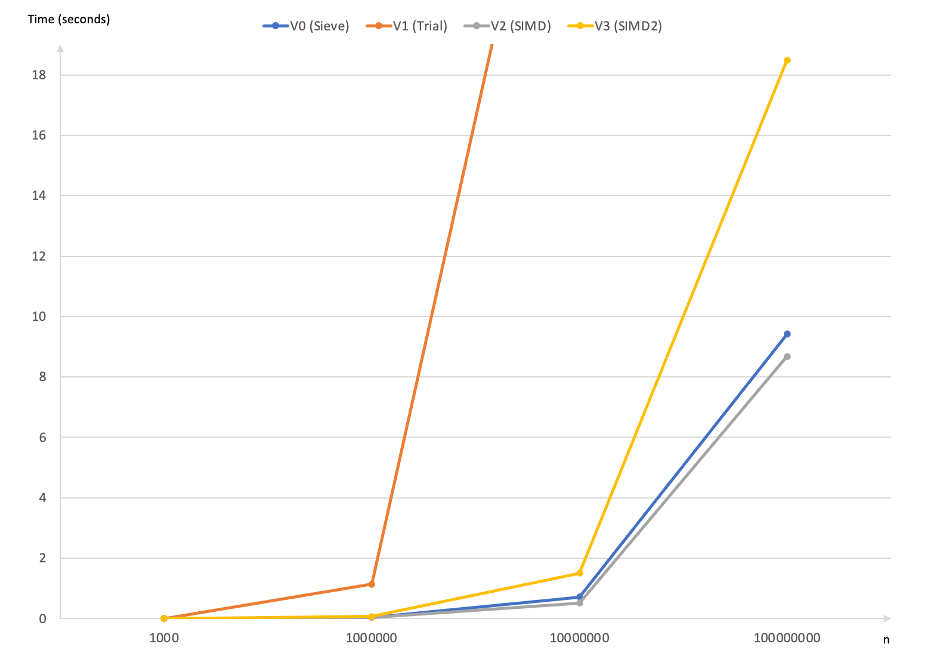
\includegraphics[width=0.9\textwidth]{images/algoperformanz.png}
\end{figure}

Für die verschiedene Eingaben wird das n jeweils als eine Potenz von 10 gewählt. 
Im ersten Testfall mit n=1'000 zeigte der Algorithmus der Probedivision im Vergleich zu den anderen Algorithmen eine deutlich schlechtere Leistung mit einer Laufzeit von 0.18ms. Da der Wert von n noch niedrig ist, war die Laufzeit für die Siebalgorithmen ähnlich: der Siebalgorithmus ohne SIMD war in 0,027ms fertig, während beide SIMD-Funktionen einen Wert von 0,035ms geliefert haben. Die Anwendung von SIMD-Befehlen hat zu einer kleiner Leistungsverringerung geführt, da zusätzliche Zeit für die Erstellung von Vektoren benötigt wurde, verglichen zur Ausführung der Berechnungen in der Sieb-Implementierung. \\
Für den Testfall n=1'000'000 zeigte der Algorithmus für die Probedivision einen deutlichen Leistungsabfall im Vergleich zu den anderen Algorithmen, nämlich 1,1 Sekunden. Die SIMD-Funktion mit Bit-Masken hat eine  Verbesserte Laufzeit mit 41.1ms geliefert so dass die ursprüngliche Siebimplementierung in gewissem Maße überwindet wurde, die 42.7ms gebraucht hat. Die zweite SIMD-Funktion war langsamer als die ursprüngliche Sieb-Implementierung mit einer Laufzeit von 74,4ms. Aus diesem Testfall kann man also schon einige Folgerungen ziehen: die Probedivision ist die langsamste Methode; die Implementation des Siebs mit SIMD zeigt keinen Performanzgewinn, sondern eine schlechtere Laufzeit verglichen zum Sieb ohne SIMD; der Performanzgewinn des SIMD Algorithmus mit Bit-Masken ist sehr gering. \\
Im nächsten Test mit n=10'000'000 wurde der Algorithmus der Probedivision aufgrund seiner langen Berechnungszeit mit 31 Sekunden als unbrauchbar eingestuft. Die Bit-Masken SIMD-Funktion konnte ihren Vorsprung mit einer Leistungsverbesserung von 31 \% gegenüber dem ursprünglichen Sieb beibehalten, 519ms im Vergleich zu 716ms. Die zweite SIMD-Funktion benötigte 2 mal so viel Laufzeit, mit 1,5 Sekunden. 
Beim letzten Test mit n=100'000'000 blieben die Ergebnisse mit den vorherigen Tests konsistent: die SIMD-Implementierung mit Bit-Masken war nach 8,67 Sekunden fertig; der Siebalgorithmus hat 9,41 Sekunden gebraucht; die zweite SIMD-Funktion zeigte eine schwache Leistung mit 18,49 Sekunden. Der Algorithmus für die Probedivision wurde bei diesem Test nicht berücksichtigt, da seine Berechnungszeit voraussichtlich 10 Minuten überschreiten würde. Letzendlich haben die Ergebniße gezeigt, dass der Algorithmus für die Probedivision im Vergleich zu den anderen Algorithmen zurückfällt, insbesondere wenn n größer als $10^6$ wird. Dies liegt an der Laufzeitskomplexität des Algorithmus wenn er durch zwei verschachtelte Schleifen implementiert wird. Die SIMD-Implementierung des Siebs durch Anwenden von Bit-Masken war der schnellster der getesteten Algorithmen, mit einer Verbesserung von 31 \% im Vergleich zur ursprünglichen Sieb-Implementierung. Immerhin ist das originale Sieb des Eratosthenes selber auch nicht deutlich langsamer; die einzige Begrenzung bei diesem Verfahren ist der Speicherbedarf.
Die zweite SIMD-Funktion war dahingegen im Vergleich zum Sieb langsamer, da diese Version eine Rechenzeit die mindestens zweifach länger war. Dies wird auf die manuelle Überprüfung der Vektorindizes und auf die erhöhte Anzahl an Speicherzugriffe zurückgeführt. Es könnte auch vermutlich möglich sein, dass der Algorithmus auf falscher Weise implementiert wurde, oder dass dieser kein richtiger Ansatz zur Optimierung des Siebs war.
\section{Zusammenfassung und Ausblick}
Zusammenfassend lässt sich sagen, dass Primzahlen ein wichtiger Teil der Mathematik und deshalb auch der Informatik sind und in vielen Bereichen Anwendung finden. In dieser Ausarbeitung haben wir die Bedeutung von Primzahlen sowie ihre Eigenschaften erläutert, und verschiedene Ansätze für die Berechnung von Primzahlen vorgestellt. Unsere Implementierungen sind zwar nicht in der Lage extrem große Primzahlen zu berechnen, jedoch muss man auch bemerken, dass der Kern für die Algorithmik der hinter der Berechnung von Primzahlen steht, eine komplexe Sache ist. Es gibt noch weitere Möglichkeiten, die Verfahren, die wir untersucht haben, weiter zu verbessern: zwei Beispiele dafür wären das Sieb von Atkin und ein segmentierter Sieb des Eratosthenes. Außerdem gibt es auch probabilistische Primzahltests, die auf Häfigkeit von Primzahlen basierend sind, wie zum Beispiel der Miller-Rabin-Test. Es wird also deutlich, dass es mehrere unterschiedliche Lösungsansätze gibt, die zur Berechnung von Primzahlen dienen. Bisher war es jedoch unmöglich, ein Muster hinter den Primzahlen zu entdecken, um den Umgang damit zu vereinfachen. Es bleiben also noch viele offene Fragen bezüglich dieser wichtigen mathematischen Entitäten zu beantworten. 
\\
\\
\\
\\
\\
\\
\\
\bibliographystyle{plain}
\bibliography{Ausarbeitung}{}
\end{document}